\chapter{Circuit Breaker}\label{ch:circuit-breaker}

\resilienceMechanismChapterIntro{Circuit Breaker}{reactive}


\section{Introduction}\label{sec:cbreaker-introduction}

The Circuit Breaker mechanism is a \textit{\enquote{resilience pattern
that prevents an application from performing an operation that is likely to fail.
By allowing it
to continue
without waiting for the fault to be fixed or wasting CPU cycles while it determines that the fault is long-lasting
}}~\cite{microsoft-cbreaker-pattern}.

When an application calls a remote service, there's always a risk of failure
(e.g., network issues, service unavailability, or timeouts).
Some of these faults are temporary (transient) and resolved quickly,
but others can be long-lasting and severe (e.g., a complete loss of connectivity, complete failure of a service).

Moreover, if a service is under heavy-load, a failure in one part of the system might lead to cascading failures.
For example, if an operation is set to time out and fail after a certain period, multiple concurrent requests could be blocked until the timeout expires.
These blocked requests consume critical resources like memory, threads, and database connections, potentially leading to system-wide failures~\cite{microsoft-cbreaker-pattern}.
In such cases, it’s more efficient for the application to quickly acknowledge the failure and handle it appropriately, rather than repeatedly retrying the operation.

\subsection{Relation to the Retry Mechanism}\label{subsec:cbreaker-relation-to-retry}

The Circuit Breaker mechanism is related to the Retry mechanism (see Chapter~\ref{ch:retry}), as both are used to handle faults that might occur when connecting to a remote service or resource.
However, the two mechanisms are used in different situations.
The Retry mechanism is used to retry an operation in the expectation that it'll succeed, while the Circuit Breaker mechanism is used to prevent an application from performing an operation that is likely to fail~\cite{microsoft-cbreaker-pattern}.

An application can combine these two mechanisms by using the Retry mechanism to invoke an operation through a Circuit Breaker.
However,
the retry logic should be sensitive to any failures returned by the Circuit Breaker
and abandon retry attempts
if it indicates that a failure is not transient~\cite{microsoft-cbreaker-pattern}.

\subsection{State Machine}\label{subsec:cbreaker-state-machine}

The Circuit Breaker mechanism works as an electrical circuit breaker~\cite{electrical-circuit-breaker},
which is a safety device that automatically stops the flow of electric current in a circuit as a safety measure
(e.g., to prevent a fire) when it detects a fault condition.
In contrast to the electrical circuit breaker which needs a manual reset,
the Circuit Breaker mechanism automatically resets itself if the fault condition is considered resolved.

The default implementation of the Circuit Breaker uses a state machine,
as illustrated in Figure~\ref{fig:circuit-breaker-state-machine}, with the following states:

\begin{itemize}
    \item \textbf{Closed} - The circuit allows the operation to execute and records its execution result
    (i.e., success or failure).
    If a configurable failure threshold is reached, the circuit transitions to the open state;
    \item \textbf{Open} - The circuit does not allow the operation to be executed.
    Instead, a predefined failure result is returned.
    The circuit remains open for a configurable period of time, after which it transitions to the Half-open state.
    This timer is used to allow the system to recover from the fault condition;
    \item \textbf{Half-Open} - The circuit allows a limited number of requests to execute the operation.
    If the combined results of these requests and the recorded ones are below the failure threshold, it is assumed that the fault causing the failure has been resolved.
    Consequently, the Circuit Breaker switches to the \texttt{Closed} state.
    If not,
    the Circuit Breaker assumes that the fault is still present,
    so it reverts to the \texttt{Open} state (restarting the timeout timer).
\end{itemize}

\begin{figure}[!htb]
    \centering
    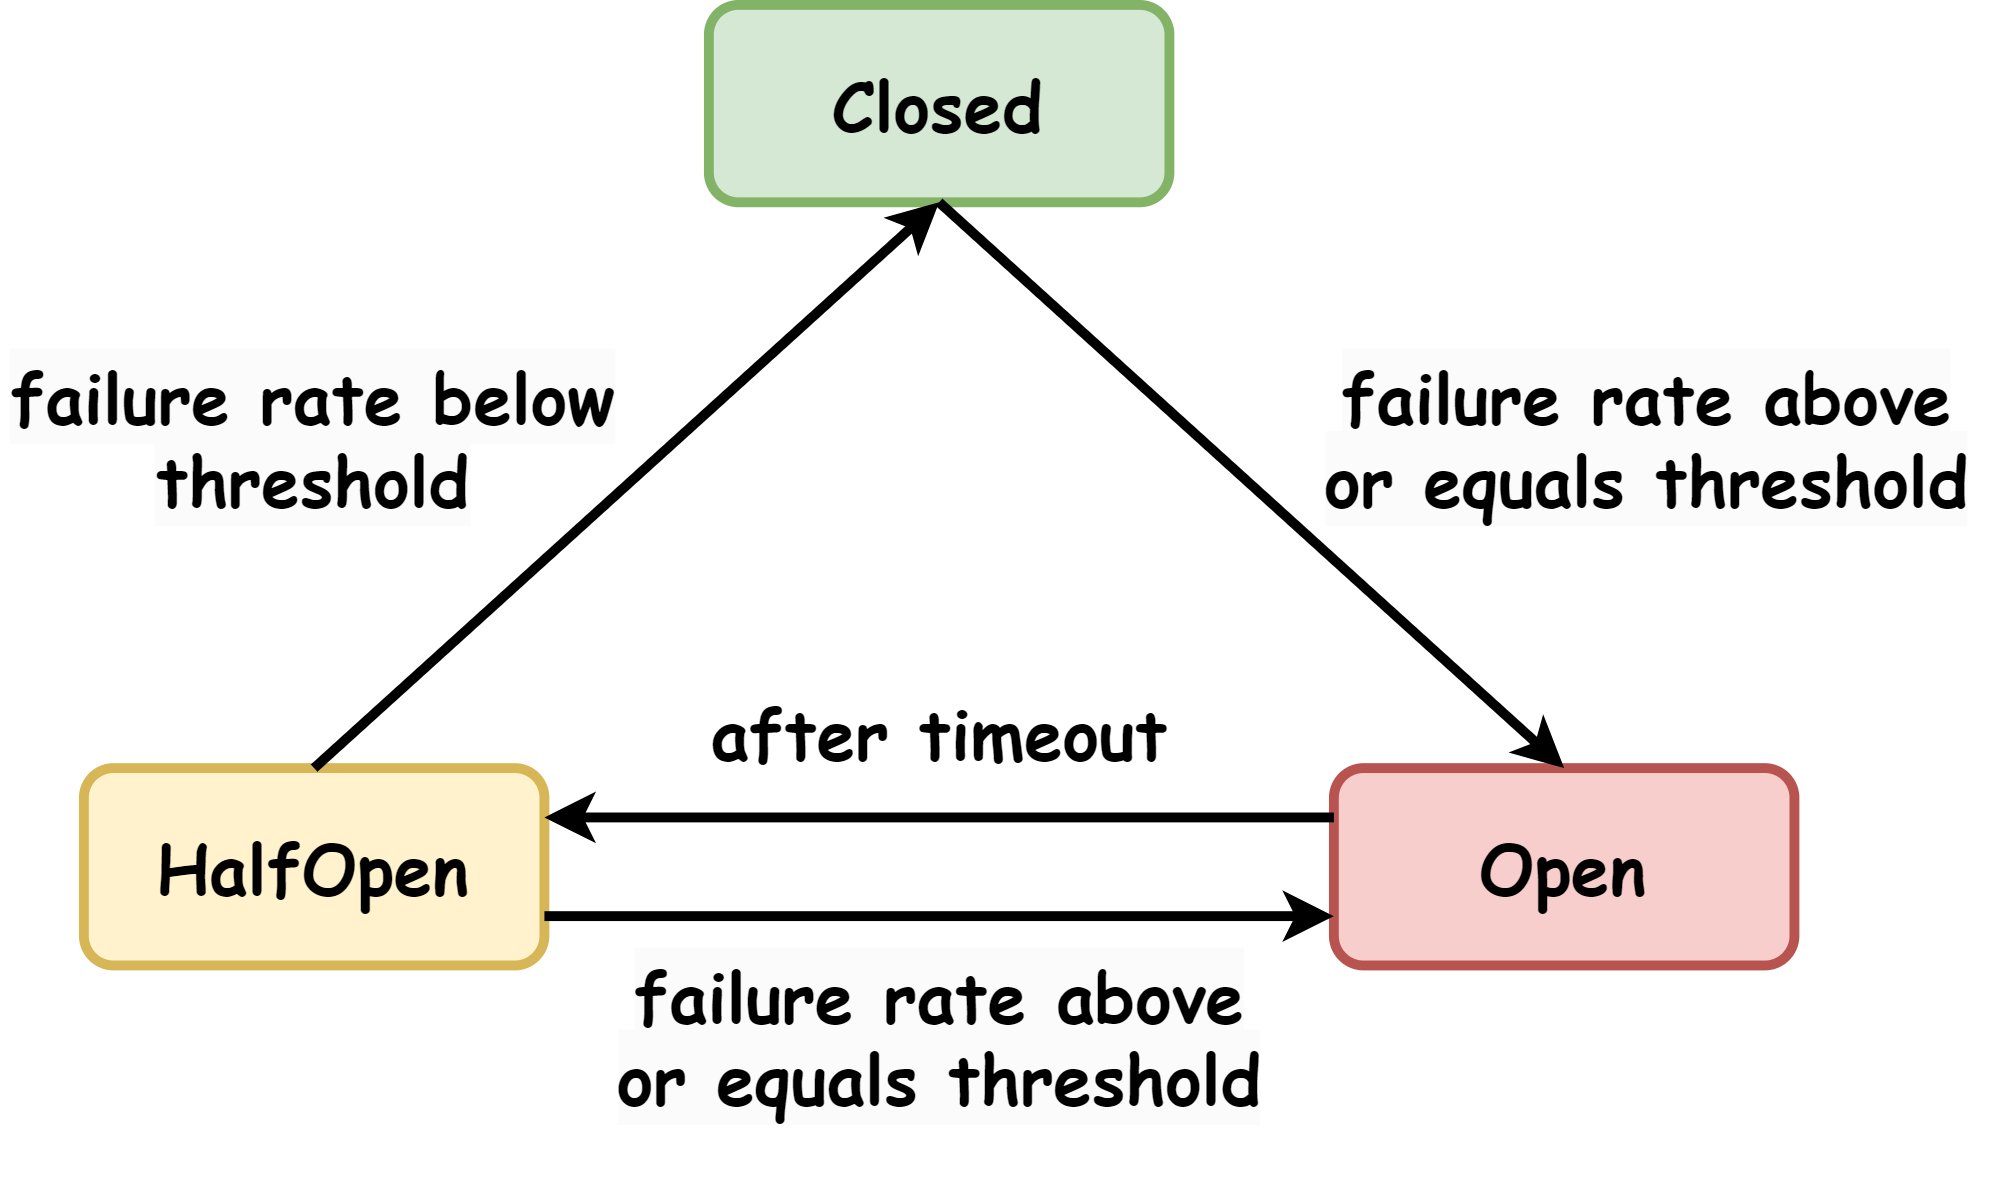
\includegraphics[width=0.6\textwidth]{../figures/05_cbreaker-states}
    \caption{Circuit Breaker State Machine.}
    \label{fig:circuit-breaker-state-machine}
\end{figure}

The \texttt{Half-Open} state is useful to prevent a recovering service from suddenly being flooded with requests.
As a service recovers, it might be able to support a limited volume of requests until the recovery is complete,
but while recovery is in progress, a flood of work can cause the service
to time out or fail again~\cite{microsoft-cbreaker-pattern}.

Other implementations might have additional states (e.g., for maintenance, testing, metrics purposes), usually manually triggered, such as:

\begin{itemize}
    \item \textbf{Forced Open} - The circuit is always open, preventing the operation from executing.
    \item \textbf{Forced Closed} - The circuit is always closed, allowing the operation to execute as if the Circuit Breaker was not present.
\end{itemize}

\subsection{Operation Execution}\label{subsec:cbreaker-operation-execution}

An operation protected by a Circuit Breaker is executed through the Circuit Breaker.
When the operation is invoked, the Circuit Breaker checks its state to determine if the operation should be executed.
The same Circuit Breaker instance can be used to protect multiple operations, sharing the same state and configuration, as illustrated in Figure~\ref{fig:cbreaker-decoration}.

\begin{figure}[!htb]
    \centering
    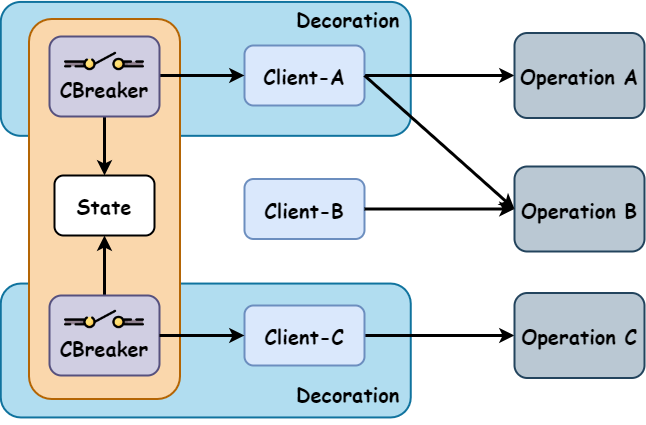
\includegraphics[width=0.6\textwidth]{../figures/05_cbreaker-decoration}
    \caption{Circuit Breaker Decoration.}
    \label{fig:cbreaker-decoration}
\end{figure}

Regarding the underlying operation execution,
it's important to note that the Circuit Breaker does not synchronize the received calls (i.e., it does not prevent multiple threads from invoking the operation concurrently when the circuit is in a state that allows the operation to be executed).
To restrict the number of concurrent calls to the operation, the Bulkhead~\cite{microsoft-bulkhead-pattern} mechanism should be used in combination with the Circuit Breaker.

\subsection{Recording Execution Results}\label{subsec:cbreaker-recording-execution-results}

The Circuit Breaker mechanism records the results of the operation executions to determine when to open the circuit.
This recording process uses a sliding window~\cite{sliding-window} which can be implemented in different ways:

\begin{itemize}
    \item \textbf{Count-based} -
    The Circuit Breaker opens when the number of failures exceeds a predefined threshold
    (e.g., 50\% of the last 10 operations failed, assuming a window size of 10).
    \item \textbf{Time-based} -
    The Circuit Breaker opens when the failure rate exceeds a predefined threshold over a specific period of time
    (e.g., 50\% of the operations failed within the last 10 seconds,
    assuming a window size of 10 with one-second intervals).
\end{itemize}

The time-based sliding window is used
to track the outcomes of recent operation executions over a specific time interval,
making decisions based on recent performance rather than solely relying on historical data
(which might not be relevant in some cases).

As newer results are recorded, older results are removed from the window, keeping a
FIFO (First In, First Out) order.
This approach ensures that the window size remains constant and that the Circuit Breaker can make decisions based on the most recent data.


\section{Implementation Aspects}\label{sec:cbreaker-implementation-aspects}

The Circuit Breaker mechanism was implemented with the following components:

\begin{itemize}
    \item \textbf{State}: Manages the Circuit Breaker state transitions and mutual exclusion;
    \begin{itemize}
        \item \textbf{Reducer} - Processes actions and updates the state accordingly;
        \item \textbf{Sliding Window} - Records the operation's execution results;
    \end{itemize}
    \item \textbf{Circuit Breaker} - Consults the state, executes operations and dispatches actions to the state reducer.
\end{itemize}

An example of the interaction between these components is illustrated in Figure~\ref{fig:circuit-breaker-execution-example},
where the Circuit Breaker receives two orderly requests to execute an operation after working for some time:

\begin{boldenumerate}
    \item Client-A requests the operation to be executed.
    As the operation is protected by the Circuit Breaker, the Circuit Breaker is consulted.
    \item The Circuit Breaker checks the shared state, in mutual exclusion,
    and sees that it is \texttt{Closed}, allowing the operation to be executed under its vigilance.
    \item The operation is executed outside mutual exclusion.
    \item The operation succeeds, and the result is recorded by the Circuit Breaker.
    Even though the operation succeeded, the minimum throughput is reached,
    and as such, the failure rate is considered.
    Since the failure rate equals the threshold, the Circuit Breaker transitions to the \texttt{Open} state.
    \item Client-B requests the operation to be executed through the Circuit Breaker.
    \item The Circuit Breaker checks the shared state, in mutual exclusion, and sees that it is \texttt{Open}, thus preventing the operation from being executed.
    \item Client-B receives a predefined failure result.
\end{boldenumerate}

\begin{figure}[!htb]
    \centering
    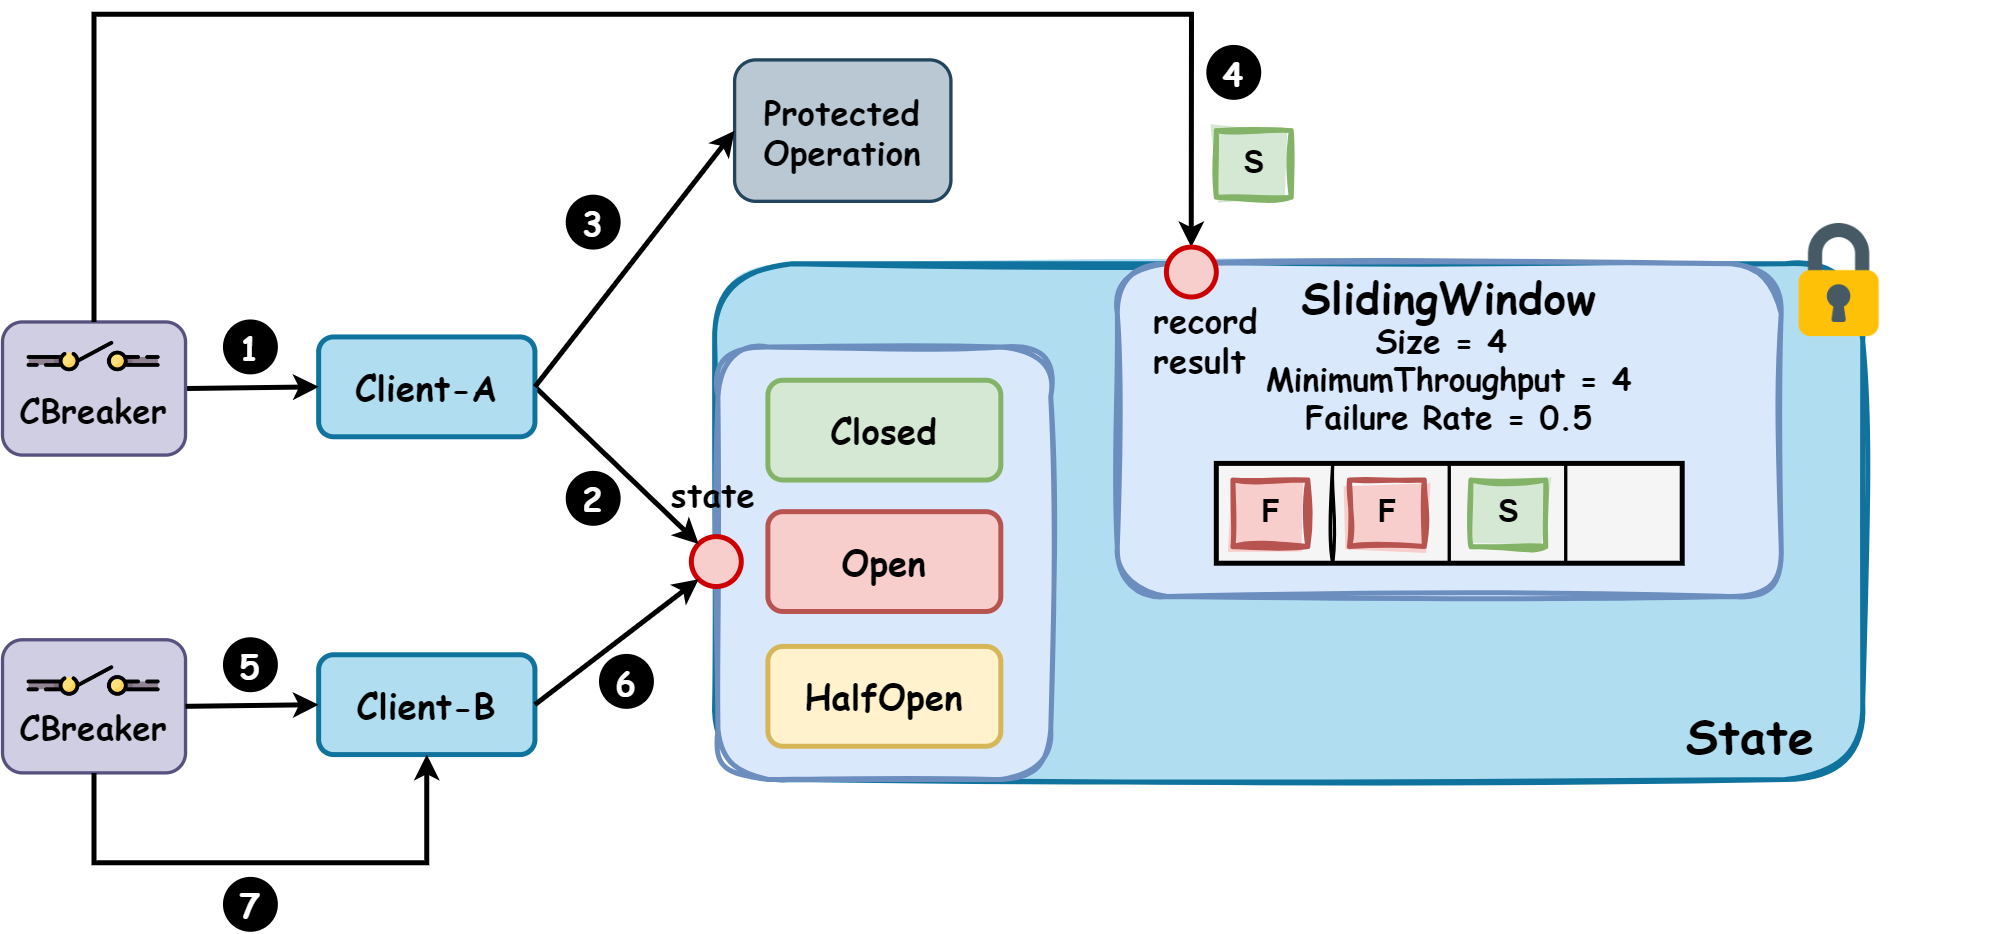
\includegraphics[width=0.8\textwidth]{../figures/05_cbreaker-execution-example}
    \caption{Circuit Breaker Execution Example.}
    \label{fig:circuit-breaker-execution-example}
\end{figure}

\subsection{State Reducer}\label{subsec:cbreaker-state-reducer}

The Circuit Breaker was implemented using the state reducer pattern,
in order to delegate the state transitions and mutual exclusion to a single component.

The reducer pattern is a design pattern
that allows the state of a system
to be managed by a single reducer function
that takes the current state and an action as input and returns the new state.
It is a common pattern in the Redux~\cite{redux} state management library and the React~\cite{react-use-reducer} library,
both widely used in the JavaScript ecosystem.

As illustrated in Figure~\ref{fig:reducer-pattern}, the reducer pattern has the following characteristics:

\begin{itemize}
    \item \textbf{State} - The state of the system is stored in a single immutable object and can be consulted as a snapshot of the system at any point in time;
    \item \textbf{Action} - An event that potentially triggers a state transition;
    \item \textbf{Dispatch} - A function that sends an action to the reducer to trigger a state transition.
    In more complex scenarios, it can also dispatch multiple actions based on a single received action, and handle side effects;
    \item \textbf{Reducer} - A function that takes the current state and an action as input and returns the new state and a list of effects (which could be empty) to be executed outside the reducer.
    This function must be a pure function, meaning it must not have side effects and return the same output for the same input (deterministic).
    \item \textbf{Effect} -
    Represents a potential side effect that is returned by the reducer as an event and handled by the dispatcher (e.g., logging, fetching external data).
\end{itemize}

\begin{figure}[!htb]
    \centering
    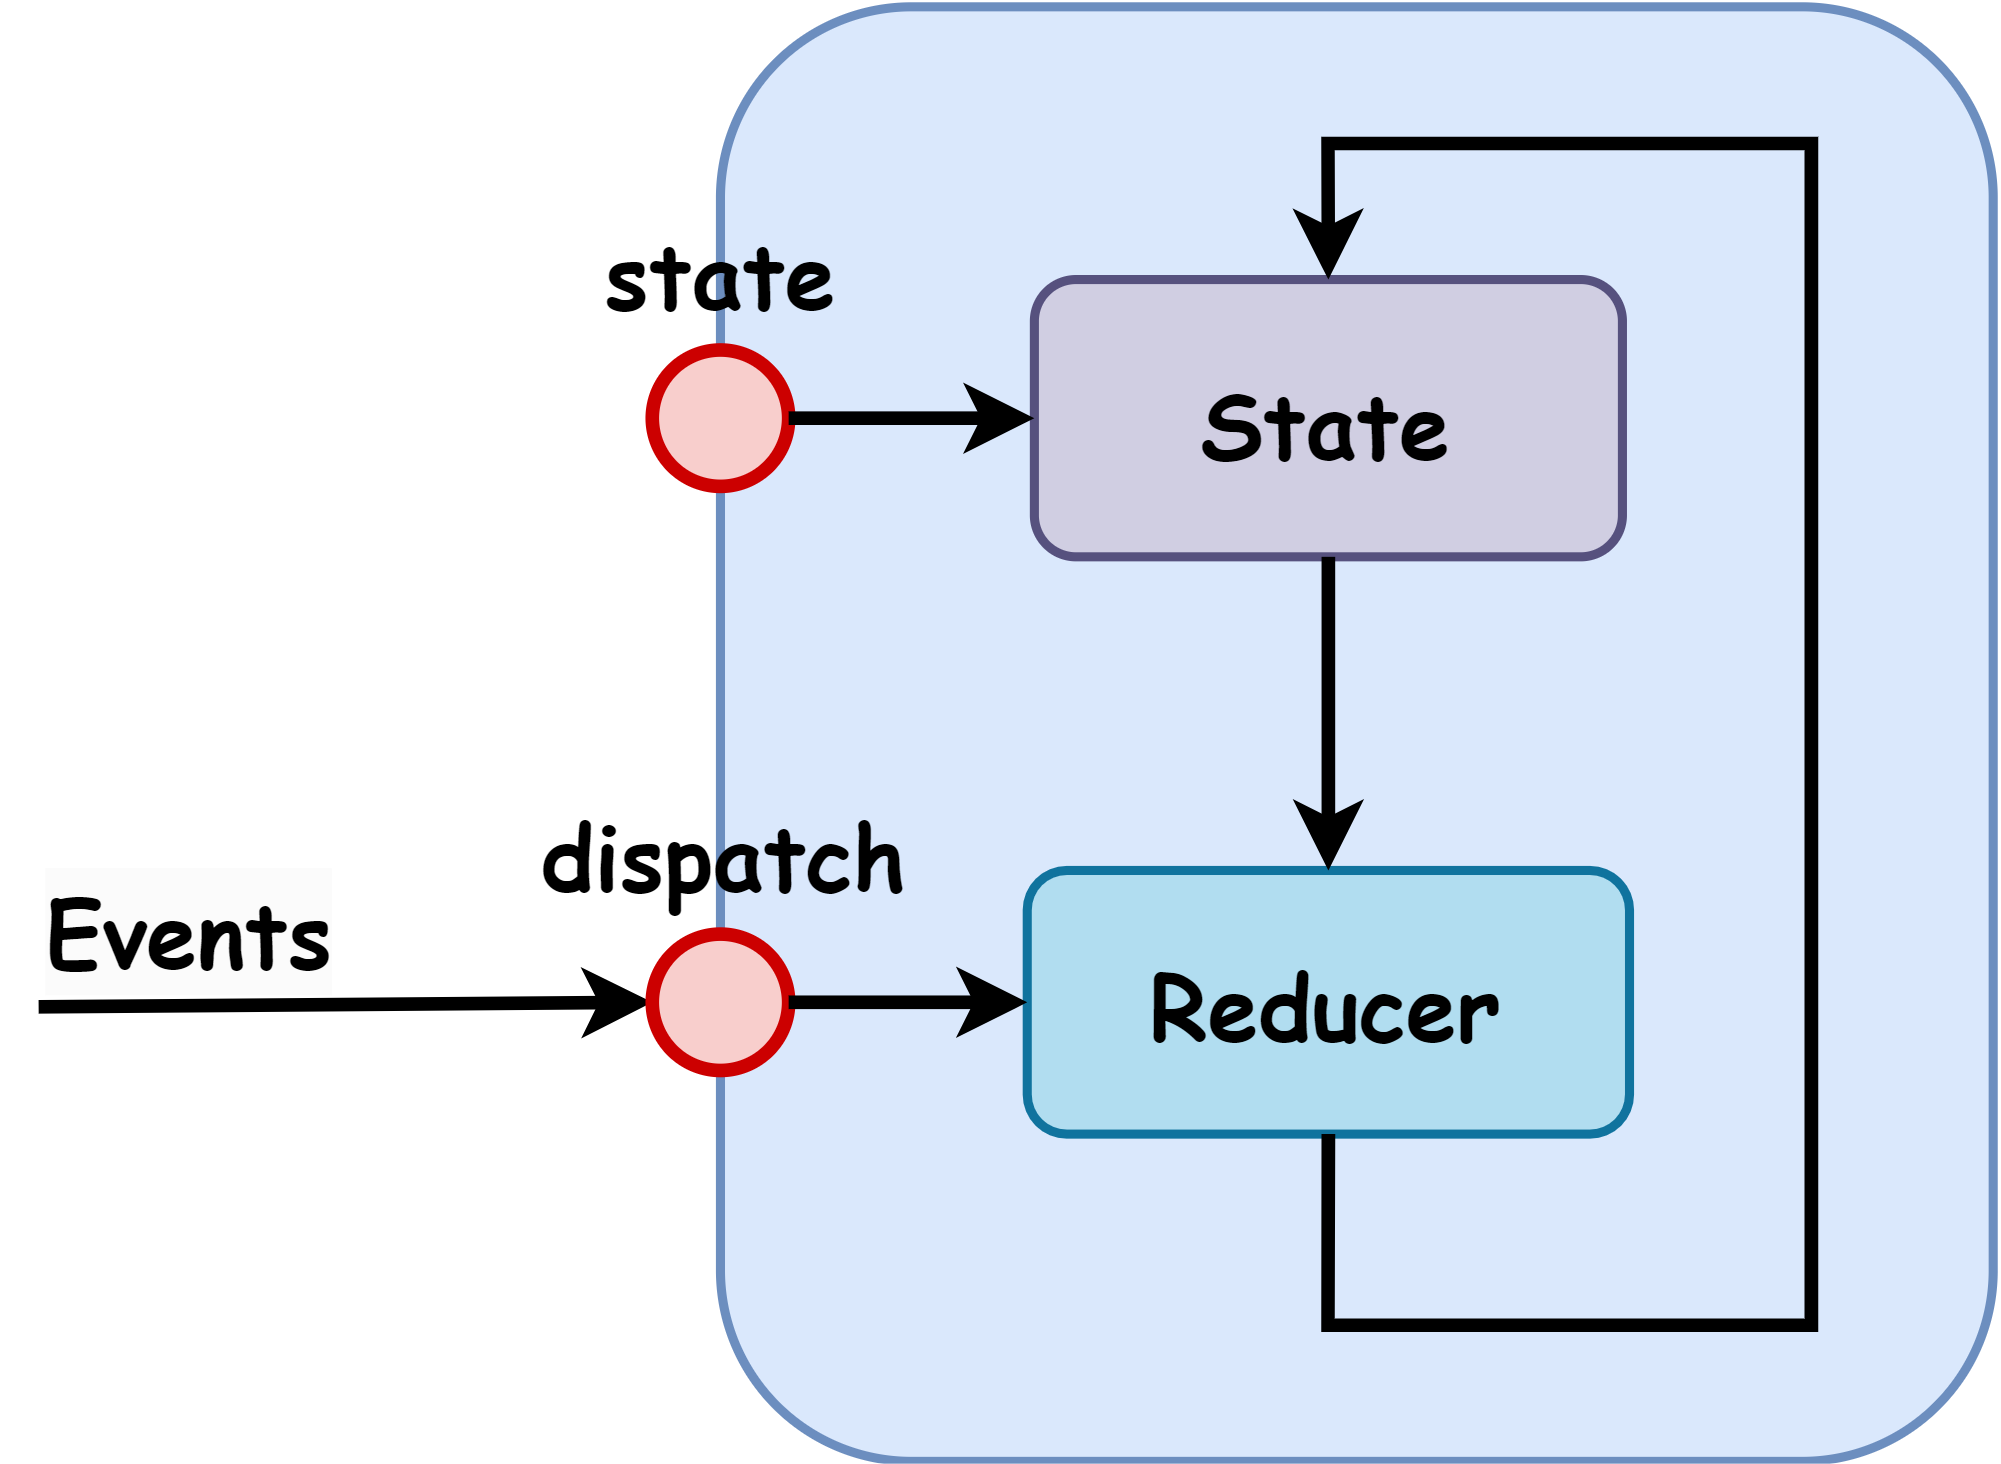
\includegraphics[width=0.5\textwidth]{../figures/05_reducer-pattern}
    \caption{State Reducer Pattern.}
    \label{fig:reducer-pattern}
\end{figure}

\subsection{Sliding Window}\label{subsec:cbreaker-sliding-window}

The sliding window, which is part of the Circuit Breaker's state, is used to record the operation's execution results and calculate the failure rate.
It is implemented as a circular/ring buffer.

A circular buffer is a fixed-size buffer with a pointer to indicate the next empty position, incrementing with each new entry.
When full, new data overwrites the oldest data, as the pointer wraps around to the beginning of the buffer, as illustrated in Figure~\ref{fig:05_circular-buffer}.
This eliminates the need to shift elements for new entries and allows for constant time complexity for adding elements~\cite{circular-buffer}.

\begin{figure}[!htb]
    \centering
    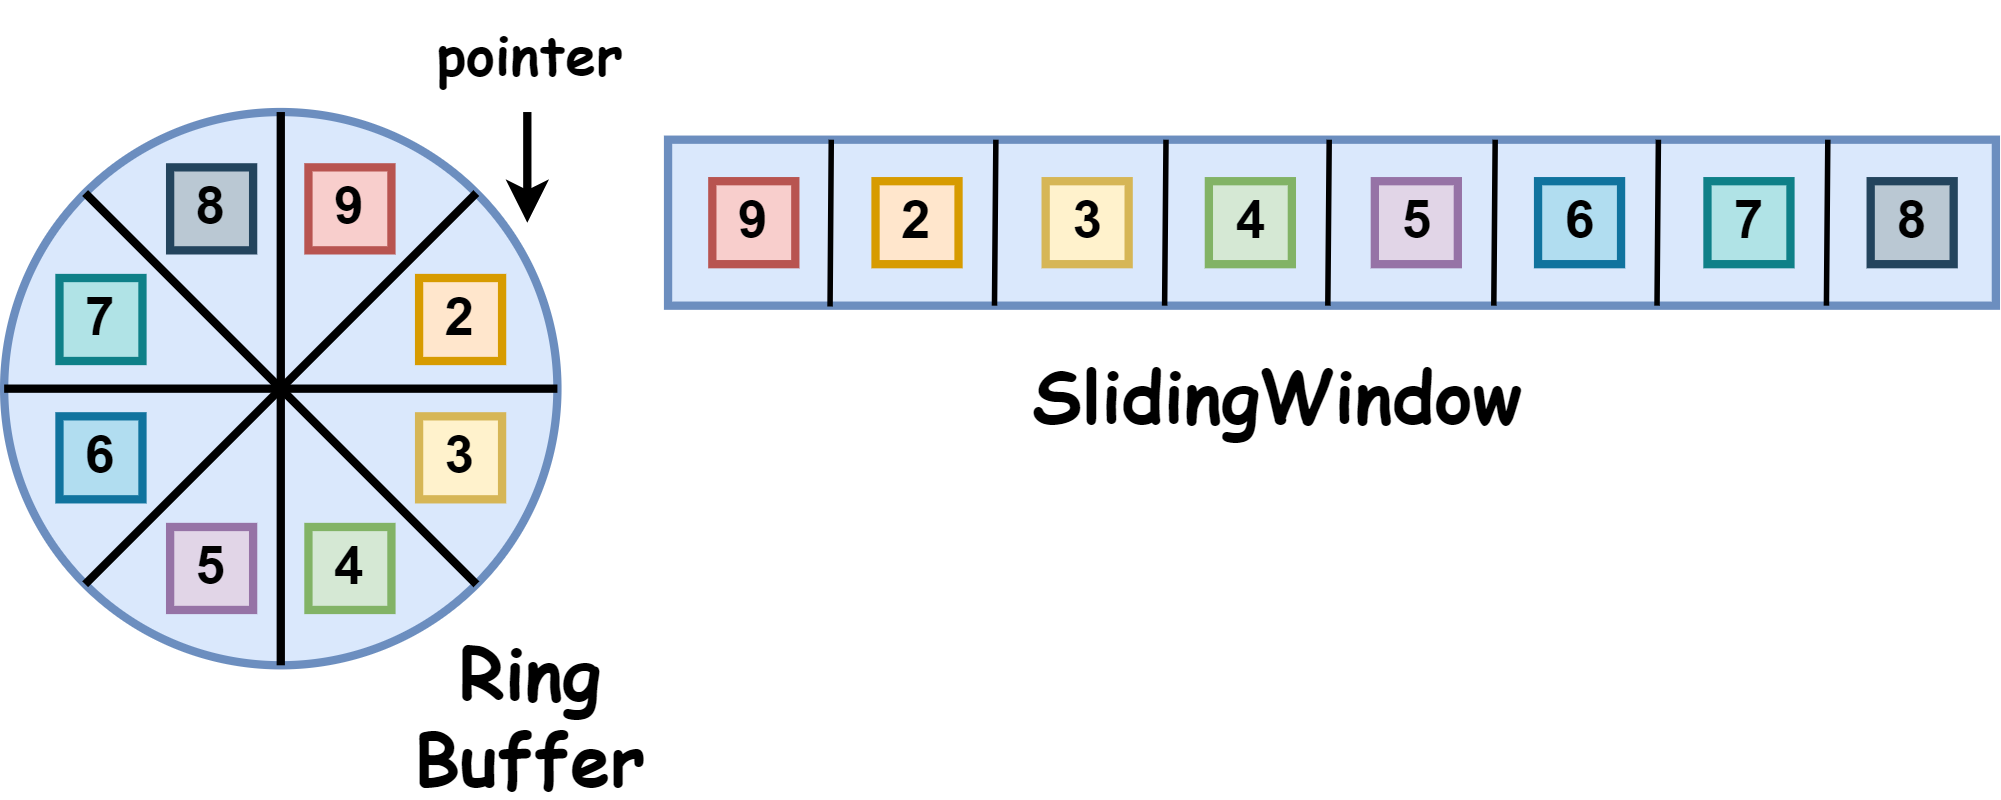
\includegraphics[width=0.8\textwidth]{../figures/05_circular-buffer}
    \caption{Circular Buffer.}
    \label{fig:05_circular-buffer}
\end{figure}

\subsection{Delay Strategy}\label{subsec:cbreaker-delay-strategy}

The delay strategy is used
to determine the duration the Circuit Breaker will remain in the \texttt{Open} state before transitioning to the \texttt{HalfOpen} state.

This mechanism presents the same delay strategy options as the Retry mechanism (See Section~\ref{subsec:retry-delay-strategies} and Section~\ref{subsec:retry-custom-delay-provider}).

\subsection{Delay Handling}\label{subsec:cbreaker-delay-handling}

The first approach to handle the delay in the \texttt{Open} state was
to launch a coroutine that transitions, after a delay, the Circuit Breaker to the \texttt{HalfOpen} state.
But this approach had two problems: handling cancellation and the reducer presenting side effects.

Instead,
a comparable time marker was used to store the exact time when the Circuit Breaker transitioned to the \texttt{Open} state.
This marker is consulted when callers send external events to the reducer component,
behaving as an internal event.
Even on state observations, the reducer component receives an event with the current time to determine if a transition is needed.
If the delay has passed, the Circuit Breaker transitions, automatically, to the \texttt{HalfOpen} state,
before attending any external events and potentially ignoring them.

The same approach was used for the \texttt{HalfOpen} state,
where the Circuit Breaker transitions back to the \texttt{Open} state
if the maximum wait duration, specified in the configuration, has passed.

\subsection{Manual State Transition and Reset}\label{subsec:cbreaker-manual-state-transition}

In later stages of the implementation, the Circuit Breaker functionality was extended to override the current state with a new state,
by allowing the caller to perform a manual state transition.
This feature was considered useful for testing, debugging,
and maintenance purposes (e.g., maintain the Circuit Breaker in the \texttt{Closed} state to only record the operation's execution results).
It's worth noting that a manual state transition maintains the same behaviour as an automatic state transition,
and won't perform any additional actions.
For example,
a transition from the \texttt{HalfOpen} state to the \texttt{Open} state will advance the delay strategy attempt counter by one.

A reset, however, places the Circuit Breaker in the \texttt{Closed} state,
clearing the sliding window and resetting the failure rate.
Effectively resetting the Circuit Breaker to its initial state.

\subsection{Retry after Rejected}\label{subsec:cbreaker-retry-after-rejected}

In some use cases, when a call is rejected by the Circuit Breaker,
it might be useful to provide the caller with information on when the operation can be retried.
In this scenario, the Circuit Breaker can return a recommended minimum
duration for the caller to wait before retrying the operation.
This duration is equivalent to the time
remaining for the Circuit Breaker to transition to the \texttt{HalfOpen} state from the \texttt{Open} state.
However, a call can be rejected by the Circuit Breaker for other reasons,
such as the permitted number of calls in the \texttt{HalfOpen} state being exceeded.
In this case, the Circuit Breaker can provide a retry-after period equivalent to the total duration of the \texttt{Open} state to give the system enough time to stabilize before the next retry attempt.

With this information,
an (outer) Retry mechanism can be configured in the pipeline before the
(inner) Circuit Breaker mechanism.
When the Circuit Breaker rejects a call,
the Retry mechanism uses the provided retry-after period to delay the next retry attempt.
Note that this behaviour, as mentioned in Section~\ref{subsec:cbreaker-relation-to-retry}, can only be possible
if the Retry mechanism is sensitive to the Circuit Breaker's rejection response.

\subsection{Event Emission}\label{subsec:cbreaker-event-emission}

The Circuit Breaker emits events to notify listeners when:

\begin{itemize}
    \item A call is rejected;
    \item The underlying operation is executed.
    Two different event types can be emitted in this case based on the operation's success or failure;
    \item The Circuit Breaker state changes manually or automatically;
    \item The Circuit Breaker is reset.
\end{itemize}


\section{Configuration}\label{sec:cbreaker-configuration}

\resilienceMechanismConfigIntroToTable{Circuit Breaker}~\ref{tab:cbreaker-config-builder}.

\begin{table}[!htb]
    \centering
    \caption{Configuration Properties for \texttt{CircuitBreakerConfigBuilder}}
    \label{tab:cbreaker-config-builder}
    \vspace{0.3cm}
    \begin{tabular}{|p{5cm}|p{5cm}|p{6cm}|}
        \hline
        \textbf{Config Property}          & \textbf{Default Value/Behaviour} & \textbf{Description}                                                                                                                                        \\ \hline
        \texttt{failureRateThreshold}     & \texttt{0.5}                     & The rate in percentage of calls recorded as failures that will trigger the Circuit Breaker to transition to the \texttt{Open} state if equaled or exceeded. \\ \hline
        \texttt{permittedNumberOfCalls InHalfOpenState} & \texttt{10} & The number of calls
        allowed in the \texttt{HalfOpen} state. \\ \hline
        \texttt{maxWaitDurationInHalf OpenState} & \texttt{0} & The maximum duration
        the Circuit Breaker will wait in the \texttt{HalfOpen} state before transitioning back to the \texttt{Open} state.
        If set to \texttt{0}, it waits indefinitely until all permitted calls are executed. \\ \hline
        \texttt{slidingWindow} & \texttt{SlidingWindow[ size=100, minimumThroughput=100, type=COUNT\_BASED]}
        & Configures the sliding window used to record calls and calculate the failure rate.
        Minimum throughput is the minimum number of calls
        that must be recorded before the failure rate is calculated.
        \\ \hline
        \texttt{delayStrategyInOpenState} & \texttt{Constant[ delay=1m]}     & The strategy used to determine the duration the Circuit Breaker will remain in the \texttt{Open} state before transitioning to the \texttt{HalfOpen} state. \\ \hline
        \texttt{recordExceptionPredicate} & \texttt{throwable ->
            true} & Predicate
        to determine if an exception thrown by the underlying operation should be recorded as a failure, and as such, increase the failure rate. \\ \hline
        \texttt{recordResultPredicate} & \texttt{result ->
            false} & Predicate
        to determine if the result of the underlying operation should be recorded as a failure, and as such, increase the failure rate. \\ \hline
        \texttt{exceptionHandler} & \texttt{Rethrow throwable
        if any} & The handler for exceptions that occur during a call through the Circuit Breaker. \\ \hline
    \end{tabular}
\end{table}

\resilienceMechanismDefaultConfig


\section{Ktor Integration}\label{sec:cbreaker-ktor-integration}

The Circuit Breaker mechanism was integrated with Ktor by implementing a custom plugin that can be added to the application's Ktor pipeline, using the implemented Circuit Breaker mechanism.

\subsection{Plugin Implementation}\label{subsec:cbreaker-plugin}

The plugin was designed for Ktor clients to wire the Circuit Breaker mechanism to the HTTP client pipeline.
The Circuit Breaker plugin will act before the request is sent to the server,
consulting the Circuit Breaker state to determine if the request should be executed and after the response is received,
recording the result of the operation.
Depending on the result, the Circuit Breaker records the operation as a success or failure.

A listener to log all events emitted by the circuit breaker context is also enabled, which cancels its subscription
when the request is completed.

\subsection{Configuration}\label{subsec:cbreaker-configuration}

The Circuit Breaker Ktor plugin can be configured
by using a dedicated configuration builder with the properties listed in Table~\ref{tab:circuit-breaker-config-builder}.

\begin{table}[!htb]
    \centering
    \caption{Configuration Properties for \texttt{CircuitBreakerPluginConfigBuilder}}
    \label{tab:circuit-breaker-config-builder}
    \vspace{0.3cm}
    \begin{tabular}{|p{5cm}|p{5cm}|p{6cm}|}
        \hline
        \textbf{Config Property}                   & \textbf{Default Value/Behaviour}                                                     & \textbf{Description}                                                                                                                                        \\ \hline
        \texttt{failureRateThreshold}              & \texttt{0.5}                                                                         & The rate in percentage of calls recorded as failures that will trigger the Circuit Breaker to transition to the \texttt{Open} state if equaled or exceeded. \\ \hline
        \texttt{permittedNumberOfCalls InHalfOpenState} & \texttt{10} & The number of calls
        allowed in the \texttt{HalfOpen} state. \\ \hline
        \texttt{maxWaitDurationInHalf OpenState} & \texttt{0} & The maximum duration
        the Circuit Breaker will wait in the \texttt{HalfOpen} state before transitioning back to the \texttt{Open} state.
        If set to \texttt{0}, it waits indefinitely until all permitted calls are executed. \\ \hline
        \texttt{slidingWindow} & \texttt{SlidingWindow[ size=100, minimumThroughput=100, type=COUNT\_BASED]}
        & Configures the sliding window used to record calls and calculate the failure rate.
        Minimum throughput is the minimum number of calls
        that must be recorded before the failure rate is calculated.
        \\ \hline
        \texttt{delayStrategyInOpenState}          & \texttt{Exponential[ initialDelay=30s, multiplier=2.0, maxDelay=10m]}     & The strategy used to determine the duration the Circuit Breaker will remain in the \texttt{Open} state before transitioning to the \texttt{HalfOpen} state. \\ \hline
        \texttt{recordResponseAsFailure Predicate} & \texttt{(response) -> records a failure if a 5xx response is received from a server}                               & Predicate to determine if a response should be recorded as a failure.                                   \\ \hline
    \end{tabular}
\end{table}

Additionally, methods relevant to an HTTP context were added to the configuration builder to simplify the configuration process:

\begin{itemize}
    \item \texttt{recordFailureOnServerErrors}:
    Records server responses with status codes in the range 500-599 as failures.
    Based on \texttt{recordResponseAsFailurePredicate};
\end{itemize}

Another feature thought to be useful was the ability
to modify the response when a call is rejected by the Circuit Breaker
(e.g., to include a Retry-After header and status code 503).
However, this feature was left as a future improvement due to time constraints.
